\documentclass{PoS}

% Shortcuts
\newcommand{\aap}{AAP}
\newcommand{\pasp}{PASP}
\newcommand{\url}[1]{\href{#1}{#1}}

\title{Gammapy -- A prototype for the CTA science tools}
\ShortTitle{Gammapy -- A prototype for the CTA science tools}

\author{
Christoph Deil$^a$,
Julien Lefaucheur$^b$,
R\'egis Terrier$^c$,
Bruno Kh\'elifi$^c$,
Matthew Wood$^d$,
Roberta Zanin$^a$,
Lars Mohrmann$^e$,
Nachiketa Chakraborty$^a$,
Jason Watson$^a$,
Rub\'en L\'opez Coto$^a$,
Stefan Klepser$^f$,
\speaker{Matteo Cerruti}$^g$,
Jean-Philippe Lenain$^g$,
Fabio Acero$^h$,
Arache Djannati-Ata{\"\i}$^c$,
Santiago Pita$^c$,
Zeljka Bosnjak$^i$,
Jose Enrique Ruiz$^j$,
Cyril Trichard$^k$,
Thomas Vuillaume$^l$,
for the CTA Consortium,
Axel Donath$^a$,
Johannes King$^a$,
L\'ea Jouvin$^c$,
Marion Spir-Jacob$^c$,
Ellis Owen$^m$,
Manuel Paz Arribas$^n$,
Brigitta Sipocz$^o$,
Dirk Lennarz$^p$
\\
\llap{$^a$}MPIK, Heidelberg, Germany\\
\llap{$^b$}LUTH, Obs. de Paris/Meudon, France\\
\llap{$^c$}APC/CNRS, Paris, France\\
\llap{$^d$}SLAC National Accelerator Laboratory, US\\
\llap{$^e$}FAU, Erlangen, Germany\\
\llap{$^f$}DESY, Zeuthen, Germany\\
\llap{$^g$}LPNHE, Paris, France\\
\llap{$^h$}CEA/IRFU, Saclay, France\\
\llap{$^i$}University of Rijeka, Croatia\\
\llap{$^j$}Instituto Astrof\'isica de Andaluc\'ia, Granada, Spain\\
\llap{$^k$}CPPM, Marseille, France\\
\llap{$^l$}LAPP, Annecy-le-Vieux, France\\
\llap{$^m$}UCL-MSSL, Dorking, United Kingdom\\
\llap{$^n$}Humboldt University, Berlin, Germany\\
\llap{$^o$}Cambridge, UK\\
\llap{$^p$}Georgia Tech, Atlanta, US\\
E-mail:
\email{Christoph.Deil@mpi-hd.mpg.de},
\email{julien.lefaucheur@obspm.fr},
\email{Roberta.Zanin@mpi-hd.mpg.de},
\email{khelifi@apc.in2p3.fr},
}

\abstract{

Gammapy is a Python package for high-level gamma-ray data analysis, written in
Python and built on Numpy, Scipy and Astropy. Starting with event lists and
instrument response information, it is possible to analyse gamma-ray data and to
create for example sky images, spectra and lightcurves, and to determine the
position, morphology and spectra of gamma-ray sources.

So far Gammapy has mostly been used to analyse data from H.E.S.S. and Fermi-LAT,
and now it is being used for the simulation and analysis of observations from
the Cherenkov Telescope Array (CTA). We have proposed Gammapy as a prototype for
the CTA science tools. This contribution will give an overview of the Gammapy
package and show analysis application examples with simulated CTA data.

}

\FullConference{35th International Cosmic Ray Conference --- ICRC2017\\
		10--20 July, 2017\\
		Bexco, Busan, Korea}


\begin{document}

\section{Introduction}
\label{sec:intro}

TODO: write me!

Astropy \cite{astropy}, Sherpa \cite{todo}, pyfact \cite{pyfact}

\section{Gammapy}
\label{sec:gammapy}

TODO: write me!

TODO: add figure with dependencies.

\section{Code example}
\label{sec:code}

An example script using Gammapy is shown in Figure~\ref{fig:code_example}.

Message: Gammapy is high-level Python, data in Numpy arrays, others have written C and Python wrappers already (WCSLib, CFITSIO, SOFA/ERFA).

\begin{figure}[t]
\centering
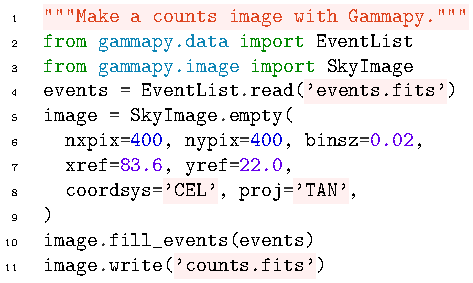
\includegraphics[width=0.5\textwidth]{examples/code_events_image}
\caption{
An example script using Gammapy to make a counts image from an event list.
This is used in Section~\ref{sec:code} to explain how Gammapy works.
TODO: probably should add a \texttt{def fill\_events(events, image)} function
and use that to illustrate how within Gammapy or in user scripts one can work
efficiently with events and pixels from Python, using Numpy arrays and
eventually calling into C extensions.
}
\label{fig:code_example}
\end{figure}


\section{Application example}
\label{sec:application}

TODO: add a CTA analysis example (probably only an image, no spectrum or
lightcurve yet). See
\url{https://nbviewer.jupyter.org/github/gammapy/gammapy-extra/blob/master/notebooks/cta\_data\_analysis.ipynb}
or if CTA-DC becomes available, a TS image from the Galactic plane survey would
be nice.

\section{Conclusions}
\label{sec:conclusions}

TODO: write me!

Briefly discuss Gammapy approach pro / con here or above?

\bibliography{gammapy-icrc2017}
\bibliographystyle{JHEP}

\end{document}
